\documentclass{article}
\usepackage[utf8x]{inputenc}

\usepackage{tikz}
\usetikzlibrary{backgrounds}

\makeatletter
\newcommand{\canvaswidth}{12}
\newcommand{\canvasheight}{6}

\newcommand{\gettikzxy}[3]{ % I got this from http://tex.stackexchange.com/questions/33703/extract-x-y-coordinate-of-an-arbitrary-point-in-tikz
    \tikz@scan@one@point\pgfutil@firstofone#1\relax
    \edef#2{\the\pgf@x}
    \edef#3{\the\pgf@y}
}
\makeatother

\tikzstyle{node}=[circle, draw, thin,fill=cyan!20, scale=0.8]

\begin{document}
    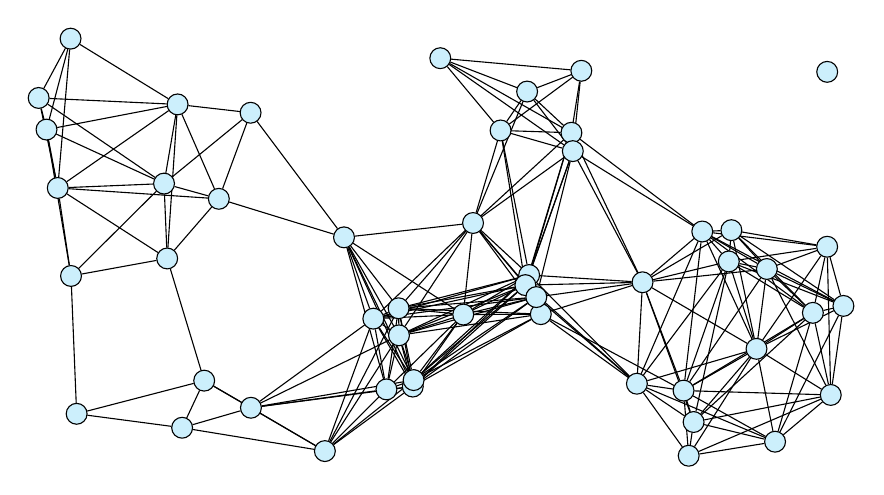
\begin{tikzpicture}
        \pgfmathtruncatemacro\nrOfNodes{50}
        \pgfmathtruncatemacro\diameter{60}

        \foreach \i in {1,...,\nrOfNodes} {
            \pgfmathsetmacro\posX{rnd*(\canvaswidth-0.6) + 0.3}
            \pgfmathsetmacro\posY{rnd*(\canvasheight-0.6) + 0.3}
            \node[node] (a\i) at (\posX, \posY) {};

            % draw node connections
            \ifnum\i>1
                \pgfmathsetmacro\last{\i -1}
                \foreach \j in {1,...,\last} {
                    \gettikzxy{(a\i)}{\pX}{\pY};
                    \gettikzxy{(a\j)}{\qX}{\qY};

                    % divide by 100 so the values are still small enough for tickz to handle while preserving adequate precision
                    \pgfmathsetmacro\diffX{(\pX-\qX)/100}
                    \pgfmathsetmacro\diffY{(\pY-\qY)/100}
                    \pgfmathsetmacro\calculatedDistance{ sqrt( (\diffX)^2 + (\diffY)^2 ) * 100};
                    \ifdim\calculatedDistance pt <\diameter pt
                        \begin{pgfonlayer}{background}
                            \draw (a\i) -- (a\j) node [midway, above, sloped] {};
                        \end{pgfonlayer}
                    \fi
                }
            \fi
        }

        %draw radio ranges
        % \begin{pgfonlayer}{background}
        %     \foreach \i in {1,...,\nrOfNodes} {
        %         \draw[color=black,fill=blue, opacity=0.05] (a\i) circle (\diameter pt);
        %     }
        % \end{pgfonlayer}
    \end{tikzpicture}
\end{document}